\documentclass[11pt,a4paper,oldfontcommands]{memoir}
\usepackage[utf8]{inputenc}
\usepackage[T1]{fontenc}
\usepackage{microtype}
\usepackage[dvips]{graphicx}
\usepackage{listings,xcolor}
\usepackage{times}
\usepackage{gensymb}
\usepackage{wrapfig}

\usepackage[
breaklinks=true,colorlinks=true,
linkcolor=blue,urlcolor=blue,citecolor=blue,% PDF VIEW
% linkcolor=black,urlcolor=black,citecolor=black,% PRINT
bookmarks=true,bookmarksopenlevel=2]{hyperref}

\usepackage{geometry}
% PDF VIEW
 \geometry{total={210mm,297mm},
 left=25mm,right=25mm,%
 bindingoffset=0mm, top=25mm,bottom=25mm}
% PRINT
%\geometry{total={210mm,297mm},
%left=20mm,right=20mm,
%bindingoffset=10mm, top=25mm,bottom=25mm}

\OnehalfSpacing
%\linespread{1.3}

%%% CHAPTER'S STYLE
%\chapterstyle{bianchi}
\chapterstyle{ger}
%\chapterstyle{madsen}
%\chapterstyle{ell}
%%% STYLE OF SECTIONS, SUBSECTIONS, AND SUBSUBSECTIONS
\setsecheadstyle{\Large\bfseries\sffamily\raggedright}
\setsubsecheadstyle{\large\bfseries\sffamily\raggedright}
\setsubsubsecheadstyle{\bfseries\sffamily\raggedright}


%%% STYLE OF PAGES NUMBERING
%\pagestyle{companion}\nouppercaseheads 
%\pagestyle{headings}
%\pagestyle{Ruled}
\pagestyle{plain}
\makepagestyle{plain}
\makeevenfoot{plain}{\thepage}{}{}
\makeoddfoot{plain}{}{}{\thepage}
\makeevenhead{plain}{}{}{}
\makeoddhead{plain}{}{}{}

\lstset{
    string=[s]{"}{"},
    stringstyle=\color{blue},
    comment=[l]{:},
    commentstyle=\color{black},
}


\maxsecnumdepth{subsection} % chapters, sections, and subsections are numbered
\maxtocdepth{subsection} % chapters, sections, and subsections are in the Table of Contents


%%%---%%%---%%%---%%%---%%%---%%%---%%%---%%%---%%%---%%%---%%%---%%%---%%%

\begin{document}

%%%---%%%---%%%---%%%---%%%---%%%---%%%---%%%---%%%---%%%---%%%---%%%---%%%
%   TITLEPAGE
%
%   due to variety of titlepage schemes it is probably better to make titlepage manually
%
%%%---%%%---%%%---%%%---%%%---%%%---%%%---%%%---%%%---%%%---%%%---%%%---%%%
\thispagestyle{empty}

{%%%
\sffamily
\centering
\Large

~\vspace{\fill}

{\huge 
Final Report
}

\vspace{2.5cm}

{\LARGE
Team Waterloop
}

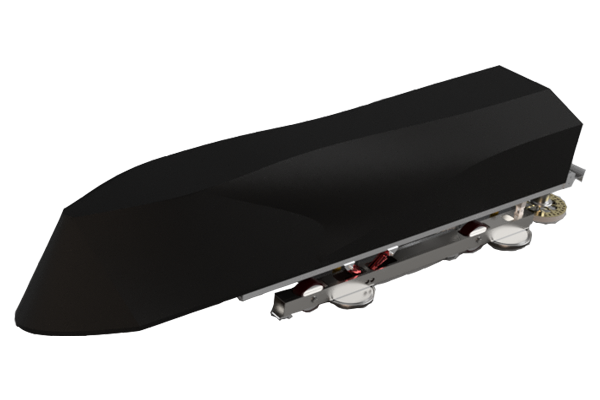
\includegraphics[width=\textwidth]{assembled_goose.png}

\vspace{3.5cm}

University of Waterloo

\vspace{\fill}

October 2017

%%%
}%%%
\clearpage
\begin{center}
This page is left blank intentionally
\end{center}
\clearpage
%%%---%%%---%%%---%%%---%%%---%%%---%%%---%%%---%%%---%%%---%%%---%%%---%%%
%%%---%%%---%%%---%%%---%%%---%%%---%%%---%%%---%%%---%%%---%%%---%%%---%%%
\begin{center}
Team Waterloop would like to recognize and thank all of our sponsors\\
put sponsors images below
\end{center}
\clearpage

\tableofcontents*

\clearpage

%%%---%%%---%%%---%%%---%%%---%%%---%%%---%%%---%%%---%%%---%%%---%%%---%%%
%%%---%%%---%%%---%%%---%%%---%%%---%%%---%%%---%%%---%%%---%%%---%%%---%%%

\chapter{Introduction}

\section{Our Goal}
Hyperloop is a new proposed form of high speed transportation that revolutionizes long distance travel. Traveling at Mach 1 on sheet of air in a low pressure tube, Hyperloop would make it possible to move between Toronto and Montreal in just 30 minutes.

In 2013, Elon Musk released a white paper discussing the technical and economic feasibilities surrounding the idea, and open-sourced the design. Musk described it as “cross between a rail gun, the Concord, and an air hockey table”~\cite{Concorde_and_airhockey}. The white paper can be accessed here. Since then, the Hyperloop Pod Competition, hosted by SpaceX, was announced to incentivize engineering teams around the world to research, design, develop, and deliver a functional half-scale prototype of a Hyperloop pod.

Waterloop is an University of Waterloo student design team. As a team in the SSDC, our primary purpose is to compete in the yearly SpaceX Hyperloop Pod Competitions. In aligning with the mission, competition pods should be designed with real-life applicability in mind. The goal of participating in the challenges set out by SpaceX is to push the development and research in the area of Hyperloop transportation. The long-term goal is to apply the knowledge gained from building a sub-scale Hyperloop competition pods to designing a real Hyperloop systems in the future.

\section{About the Team}
Waterloop is a team of ambitious students from the University of Waterloo who have been researching and developing a prototype Hyperloop pod since September 2015 to compete in the SpaceX Hyperloop Pod Competitions. We are one of two Canadian teams remaining in the competition and one of only 31 teams remaining from the initial 1200+ teams.

The team is based in Waterloo, Ontario, Canada’s largest high tech innovation hub. Our location makes it possible to access a variety of unique services, such as LOT41 Technology and Arts Campus, 3D printing from Communitech start-up Inksmith, and the Waterloo Institute for Sustainable Energy.

Waterloop is different than most University of Waterloo student teams in that we are comprised of a diverse set of students from a number of faculties. We have a substantial number of engineering students driving the design of pod subsystems, but we also have a number of students specializing in architecture, physics, computer science, business, and finance. We are a passionate team united with the common goal of building a pod that wins competitions and can scale up to become a feasible method of transportation in Canada.

We are excited to work on technology that has never existed before and which has potential to greatly improve the quality of life for people around the world. We’re very proud to be actively promoting improved transit infrastructure in Canada which can bring people together and link our local economies, while simultaneously reducing traffic, energy use, and emissions. Our goal is to create a solution that will eliminate the reliance on fossil fuel based modes of transportation for both industry and transit in a convenient and economical way. Most importantly, we wish to demonstrate feasibility of Hyperloop technology for adoption in Canada and be at the frontier of bringing Hyperloop to reality.

\subsection{Team Members}
list of all team members in here

\section{History}
\begin{itemize}
    
    \item Summer 2015:
    \begin{itemize}
        \item Assemble the Team.
        \item Officially registered as a University of Waterloo Student Engineering Team.
    \end{itemize}
    
    \item Fall 2015:
    \begin{itemize}
        \item Preliminary design briefing and evaluation by SpaceX. One of the 1200 teams entering the competition.
    \end{itemize}
    
    \item Winter 2016:
    \begin{itemize}
        \item Final design briefing and evaluation by SpaceX.
        \item Hyperloop Design Weekend at Texas A\&M. One of the 31 teams around the world to advance.
    \end{itemize}
    
    \item May 2016:
    \begin{itemize}
        \item Subsystem R\&D and feasibility analysis.
        \item Granted a private workshop at the Sedra Smith Design Centre at the University of Waterloo.
    \end{itemize}
    
    \item June 2016:
    \begin{itemize}
        \item Designing and building rigs for subsystem testing - air levitation, eddy current braking, operating electronics in a vacuum.
    \end{itemize}
    
    \item August 2016:
    \begin{itemize}
        \item Parts sourcing.
        \item Frame fabrication.
        \item Construction of a low speed test track.
        \item Finalizing Goose I subsystem design.
    \end{itemize}
    
    \item October 2016:
    \begin{itemize}
        \item Achieved air levitation.
        \item Development of embedded and communication systems.
        \item Vacuum chamber testing.
        \item Launching a Kickstarter campaign to supplement sponsorship.
    \end{itemize}
    
    \item November 2016:
    \begin{itemize}
        \item Successfully raised CA\$43,416 with 507 backers on Goose I Kickstarter campaign.
    \end{itemize}
    
    \item December 2016:
    \begin{itemize}
        \item High speed performance testing
        \item System optimization.
        \item Reliability and safety testing.
    \end{itemize}
    
    \item January 2017:
    \begin{itemize}
        \item Attending SpaceX competition with Goose I pod. (Which one?)
    \end{itemize}
    
    \item February 2017:
    \begin{itemize}
        \item Analyzing feedback from the SpaceX competition.
    \end{itemize}
    
    \item March 2017:
    \begin{itemize}
        \item Beginning the build of Goose II pod. Working on overall system improvements and overhaul of multiple subsystems based on feedback from competition.
    \end{itemize}
    
    \item May 2017:
    \begin{itemize}
        \item Developing a brand new embedded and communication systems.
        \item Completing the assembly of Magnetic Wheels for Goose II.
        \item Starting Goose II shell design process.
        \item Starting the final assembly of the pod.
    \end{itemize}
    
    \item June 2017:
    \begin{itemize}
        \item Vibrational testing of the Goose II to find and eliminate any resonance frequencies.
        \item Testing new embedded systems elements in vacuum.
        \item Integrating required sensors into embedded systems.
        \item Testing communication systems and data visualization on front-end.
        \item Completing static and dynamic levitation tests.
    \end{itemize}
    
    \item July 2017:
    \begin{itemize}
        \item Goose II unveil.
        \item Beginning preparations for SpaceX Competition 2.
        \item Implementing redundancy checks and safety enhancing features in software.
        \item Second vibrational testing to tune shock absorption for competition.
    \end{itemize}
    
    \item August 2017:
    \begin{itemize}
        \item Tuning speed controllers for Magnetic Wheels.
        \item Finalizing internal wiring of the pod.
        \item Completing required administrative arrangements for the competition and transportation of the pod to SpaceX headquarters in California.
        \item Major Mcdonald's run.
        \item Shipping the pod to California.
        \item Attending SpaceX Competition 2.
    \end{itemize}
    
\end{itemize}

\chapter{Design}

\section{High-level Design overview}
As part of the SpaceX competition, team Waterloop had developed a complete solution for the pod as well as the entire infrastructure build around the vehicle, excluding the competition test track, which is in the SpaceX HQ in California.
The entire pod is based on six major subsystems: Electrical, Software, Levitation, Shell, Propulsion, and Brakes.
Goal of Team Waterloop from the day of the team initiation is to design a complete and cost-efficient Hyperloop pod. To develop the appropriate solution, X major design challenges had to be solved in the pod design process:
\begin{itemize}
 \item frictionless propulsion, 
 \item lateral stability, 
 \item levitation, 
 \item control system,
 \item add more here…
\end{itemize}
After thorough design process and the lessons learned from Goose 1 pod, team Waterloop has developed and tested a complete competition ready vehicle to be raced in the SpaceX’s Hyperloop 1-mile long test track. \\

The pod utilizes air bearings for the levitation system, the design allows only for a minimal levitation from the ground, however eliminates most of the friction. Four air bearings are evenly spaced around the pod skis to ensure even air release and consistent levitation margin.  \\

INSERT A CAD IN HERE\\

To support the air bearings levitation system i.e. to provide a consistent release of air the pod stores all of the compressed air reserves in two tanks located in the middle of the pod body. In addition, to storing air in air tanks, team Waterloop designed complete pneumatic circuitry that supplies the air reserves to the air skis and other pneumatic components.\\

To ensure lateral stability and a provide pod with propulsion team Waterloop has developed magnetic wheels that are based on the principles of a Halbach array~\cite{Halbach_Array}.

\section{Levitation}

\subsection{Pneumatic Circuit}

\subsection{Levitation Skis}

\section{Propulsion}

\subsection{Magnetic Wheels}

\subsection{Emergency Drive}

\section{Software}
The entire software sub-system is based on three components: embedded systems, communication systems, and front-end. Embedded-systems is responsible for all of the pod's internal communications with the sensors, low-level control of the sub-systems, and various basic safety checks. Communication-systems is responsible for the transport of information from the vehicle to the front-end to allow for live data visualization and remote control of the pod. Front-end is responsible for displaying all of the pod's vital readings and providing an interface to control the pod while in the tube. All of the code written for the software system of the pod is available for public access at \href{http://www.sharelatex.com}{Waterloop's Github Page}

\subsection{Embedded Systems}

\subsubsection{Infrastructure}
Goose II uses an Arduino Mega 2560 as the main processing unit. The decision criteria for the hardware was as follows:

\begin{itemize}
    \item Familiar development language and environment
    \item Accessible I/O pin-out
    \item Support for off-the-shelf sensors and electrical components
    \item Support for custom watchdog and access to non-volatile memory
    \item Performance considerations
    \item Ability to function in a vacuum environment
\end{itemize}
\clearpage

Two boards were mainly considered as the main computing engine for the embedded systems: Arduino Mega  and STM32F746ZG. 

\bigskip
\begin{minipage}{\textwidth}
\begin{center}
\begin{tabular}{ |c||c|c| } 
 \hline
 & Arduino Mega 2560 & STM32F746ZG\\
 \hline\hline
 Processor & ATmega2560 & ARM® 32-bit Cortex®-M7 CPU \\ 
 \hline
 Clock Speed & 16 MHz & up to 216 MHz \\ 
 \hline
 Operating Voltage & 5 V & 3.3 V \\ 
 \hline
 Max Operating Temperature & +85 \degree C & +85 \degree C \\ 
 \hline
 GPIO & 54 \footnote{The GPIO in AT-Mega 2560 is expandable with a third-party shield} & Up to 144 \\ 
 \hline
 Flash Memory & 256 KB \footnote{256 KB of which 8 KB used by bootloader} & 1 MB \\ 
 \hline
\end{tabular}
\end{center}
\end{minipage}
\bigskip

While the STM32F746ZG is a more powerful option, Arduino Mega 2560 offers easier and more familiar development environment with support for C++ and also provides an unparalleled integration with the off-the-shelf components.

When designing embedded system infrastructure, the team was challenged to create reusable code modules that will allow for easier transfer of knowledge. The following challenge is crucial to long-term support of the developed embedded-systems infrastructure, as Waterloop is a student design team with fairly high turnover rate of members due to factors such as mandatory co-op terms and graduation of senior students. As a result, all of the code for Arduino is written in C++14 with an extension to compile modular files into a single Arduino executable object using Platformio. By creating a modular development environment, the team is capable of reusing developed software such as custom created libraries for specific sensors installed on the pod.

\subsubsection{Safety Measures}
Goose II has a list of safety measures that are implemented at all levels starting from electrical circuits to the front-end controls. Embedded-systems are responsible for two major safety features:
\begin{itemize}
    \item Watchdog - In order to avoid process blocking behaviour and work around the low performance of Arduino Mega 2560 that would result in delay of command execution or complete loss of control of the pod, team Waterloop has developed a custom watchdog for the embedded-systems. In case, when the CPU's processing power is exhausted and it does not respond in appropriate time frame, a watchdog gets triggered that resets the Arduino.
    \item Self recovery - In order to come back to a functioning state after a reset be it due to a triggered watchdog or due to a temporary loss of power, Arduino's non-volatile memory is used to store the state of the pod at all times, which allows the pod to come back to a fully functioning state even after a complete reset of the Arduino board.
    \item Command Received Check - To ensure that the commands sent from the front end have successfully been shipped to the Embedded systems and executed, Arduino generates a response message upon every command's arrival and upon its execution.
    \item Heartbeat Check - In order to check the state of interaction between front-end and Arduino, a heartbeat can be issued upon request from the front-end controls.
\end{itemize}

\subsection{Communication System}
\subsubsection{Infrastructure}
Three major design decisions had to be made in order to develop a powerful and flexible communication pipeline to transfer packets from the low-level Arduino environment to a high-level front-end. (1) Enabling wireless connectivity for Arduino. (2) Creating an advanced data transfer channel with limited Arduino capabilities. (3) Creating an abstract package that structure that allows for transfer of various data types without an overhead cost. The following are the criteria that have to be satisfied in a perfect communication pipeline design.

\begin{itemize}
    \item Familiar development language and environment
    \item Wireless data transfer from the low-level Arduino environment to a high-level front-end
    \item Channel that allows for a fast and high volume transfer of data
    \item Standardized message packets
\end{itemize}

A design decision has been made to use websocket based communication for bilateral communication pipeline with low delay and high channel capacity. In addition, TCP based control system allows to monitor packages arrival.

Due to the lack of extra processing power in Arduino to handle high-level data transfer methods such as websockets, an external device has been added to the communication-system to take the load of data transfer form Arduino. See below for the entire diagram of the communication-system.

\bigskip
\begin{figure}[htbp]
\centering
\fbox{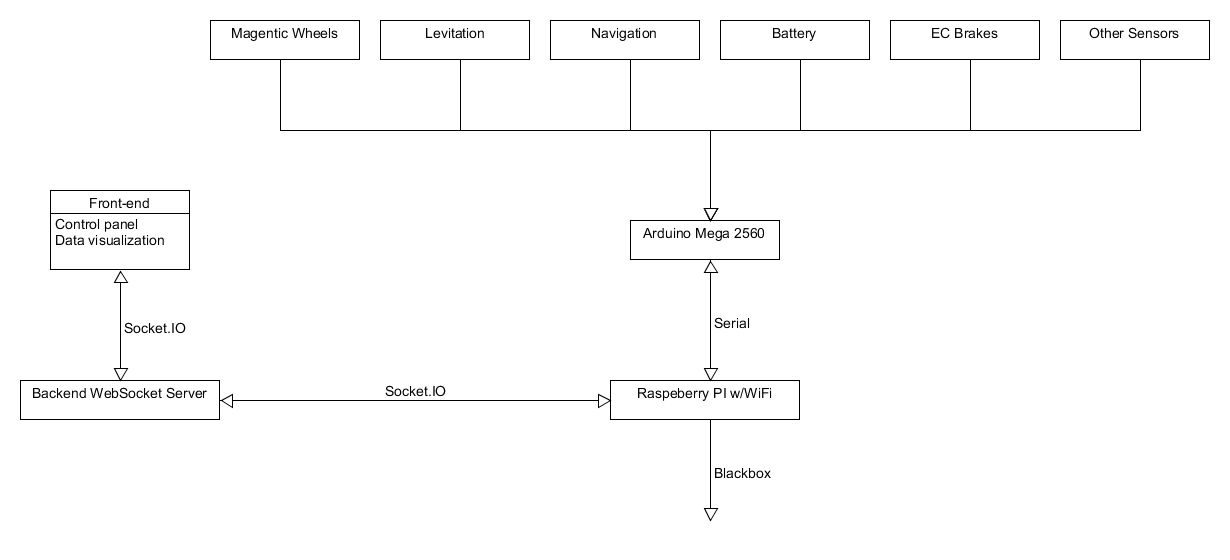
\includegraphics[width=\textwidth]{comm_pipeline.png}}
\caption{\label{fig:comm_pipeline} Goose II Communication Pipeline}
\end{figure}
\bigskip

The addition of an independent processing device for data transfer allowed for modularity of the embedded and communication systems. An abstract JSON structure with custom fields for two types of communication packages, a command and a message, have been developed to further support the concept of modularity and allow for zero additional package processing by the communication pipeline software.\\

An example of an abstract JSON command:
\bigskip
\begin{lstlisting}
{
    "cmd": "emg",
    "val": [0]
}
\end{lstlisting}
\bigskip

The parameter "cmd" describes the type of control command to be executed. The parameter "val" specifies the the state to be set as active. Please see \ref{appendix:comm_messages} for all communication pipeline commands.\\

An example of an abstract JSON message:
\bigskip
\begin{lstlisting}
{
    "time":1009,
    "sensor":"gyro",
    "data":[-1.54875,12.19750,11.36625, 1]
}
\end{lstlisting}
\bigskip

The parameter "time" describes the timestamp of the message sent from Arduino. The parameter "sensor" specifies the sensor which emitted the message. The parameter "data" specifies the data to be sent. Please see \ref{appendix:sensor_messages} for all communication pipeline messages.\\

\subsubsection{Features}
\begin{itemize}
    \item Blackbox - Due to a larger capacity of non-volatile memory on Raspberry PI, the feature of a blackbox has been implemented, where every command and sensor reading sent from Arduino to Raspberry PI is logged in a file.
    \item Data Logging - In addition to Blackbox functionality, a separate file is generated by the pod with all of the sensor readings. Such file proved to be very useful during testing to analyze patterns in vibrations and resonance frequencies, as well as post data processing such as velocity to wheel rpm ratios.
\end{itemize}

\subsection{Front end}

\subsection{Software system integration}

\section{Electrical}

\subsection{Sensors}

\subsection{Circuit}

\section{Brakes}

\section{Shell}

\chapter{Testing}

\section{Vacuum Testing}

\appendix

\chapter{Appendices}

\section{Control Communication Pipeline Packages}
\label{appendix:comm_messages}

\begin{center}
    \begin{tabular}{ |c|c|c|c| }
         \hline
            \textbf{Command Name} & \textbf{Command Code} & \textbf{Values Allowed} & \textbf{Example command} \\
         \hline\hline
            EC Brake & "brk" & 0 / 1 & \{"cmd":"brk","val":[0]\} \\ 
         \hline
            Emergency & "emg" & 0 / 1 & \{"cmd":"emg","val":[0]\} \\ 
         \hline
            Speed & "spd" & 0 - 100 & \{"cmd":"spd","val":[50]\} \\ 
         \hline
            Mode & "mode" & 0 / 1 / 2 & \{"cmd":"mode","val":[0]\} \\ 
         \hline
            Ball Valve & "bv" & 0 / 1 & \{"cmd":"bv","val":[0]\} \\ 
         \hline
            Heartbeat & "check" & 0 / 1 & \{"cmd":"check","val":[1]\} \\  
         \hline
            Save State & "rest" & 0 / 1 & \{"cmd":"rest","val":[0]\} \\
         \hline
            Stop Pod & "stop" & 0 & \{"cmd":"stop","val":[0]\} \\  
         \hline
            Start Pod & "start" & 0 & \{"cmd":"start","val":[0]\} \\  
         \hline
    \end{tabular}
\end{center}

\section{Message Communication Pipeline Packages}
\label{appendix:sensor_messages}

\begin{center}
    \begin{tabular}{ |c|c|c| }
        \hline
        \textbf{Message Type} & \textbf{Example Message}\\
        \hline\hline
        Sensor  & \{"time":1009,"sensor":"gyro","data":[-1.54875,12.19750,11.36625,1]\}\\ 
        \hline
        Command Received & \{"time":2309,"received":"{"cmd":"emg","val":[0]}"\} \\
        \hline
        Message & \{"time":4037,"message":"Setup has been called"\} \\
        \hline
    \end{tabular}
\end{center}

\bibliographystyle{unsrt}
\bibliography{waterbib}

\end{document}

